
\begin{align}
    \tag{23.1}
    f_{Y}(y) = \int_{-\infty}^{\infty}f_{X,Y}(x,y).dx
\end{align}
\begin{align}
    \tag{23.2}
    \implies f_{Y}(y) = \left\{
    \begin{array}{ll}
      0+\int_{0}^{1-y}2.dx & 0\leq y\leq 1 \\
      0 & otherwise \\
    \end{array} 
    \right.
\end{align}
\begin{align}
    \tag{23.3}
    \implies f_{Y}(y) = \left\{
    \begin{array}{ll}
      2(1-y) & 0\leq y\leq 1 \\
      0 & otherwise \\
    \end{array} 
    \right.
\end{align}
\begin{align}
    \tag{23.4}
    \therefore f_{Y}(1/2) = 1
\end{align}
\begin{figure}
\centering
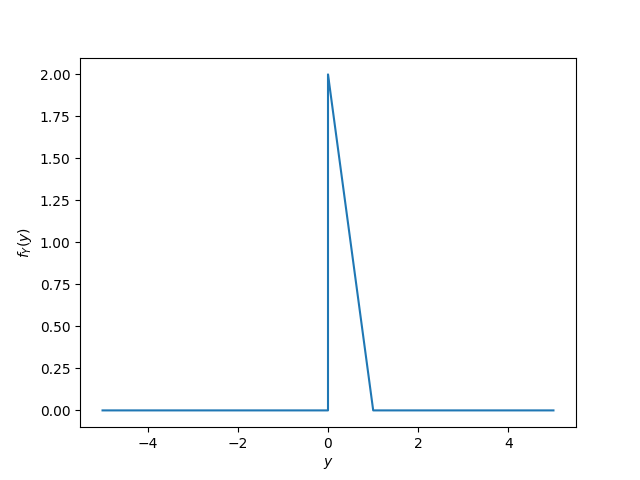
\includegraphics[width=\columnwidth]{solutions/ma/2018/23/Figure/Plot.png}
\caption{Marginal PDF}
\label{fig:ma2018-23:marginal}
\end{figure}


